\section{Échanges MAVLINK natifs implémentés}
\subsection{Heartbeat}
Nous utilisons le message HEARTBEAT pour annoncer l'existence d'une caméra sur le réseau MAVLink, ainsi que son ID système.

Le HEARTBEAT permet au système maître de découvrir les équipements connectés au réseau et d'en déduire lorsqu'ils se sont déconnectés. Un système est considéré comme étant connecté au réseau si son message HEARTBEAT est régulièrement reçu, et déconnecté si un certain nombre de messages attendus ne sont pas reçus.

\subsection{Camera Informations}
\begin{figure}[ht]
    \centering
    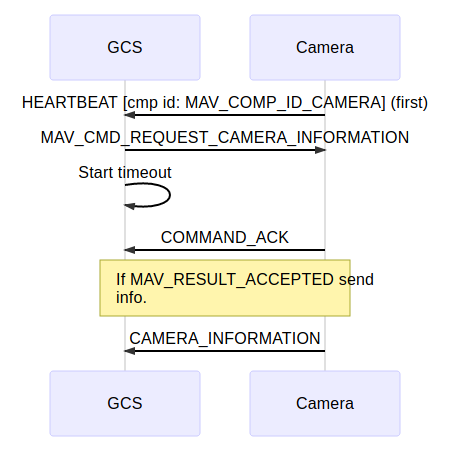
\includegraphics[scale=0.65]{img/camera_informations.png}
    \caption{Diagramme de demande d'informations}
    \label{fig:CameraCmdInfoExch}
\end{figure}

La station de contrôle doit suivre les étapes comme sur la figure ci-dessus pour obtenir les informations générales de la caméra. 

CAMERA\_INFORMATION est un message MAVLINK 2 contenant une structure avec les informations suivantes : 
\newpage
\begin{figure}[ht]
    \hspace{-2cm}
    {
        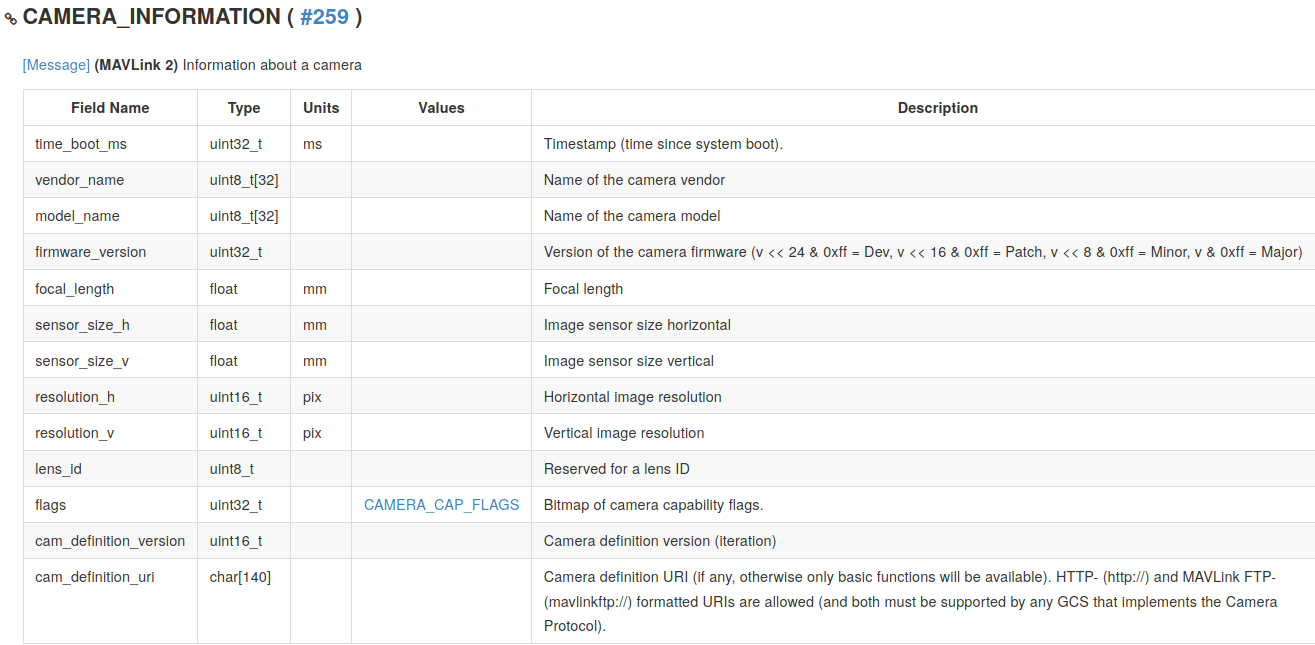
\includegraphics[scale=0.39]{img/camra_info_structure.png}
    }
    \caption{Champs des informations de la caméra}
    \label{fig:Camerainfostruct}
\end{figure}
%\begin{table}[ht]
%    \centering
%    \begin{tabular}{|c|c|c|c|l|}
%        \hline
%        Field Name    & Type   & Units  & Values & Description\\
%        \hline
%        time\_boot\_ms      & uint32\_t     & ms    & -     & Timestamp (time since system boot).\\
%        \hline
%        mode\_id	      & uint8\_t     & -    & CAMERA\_MODE     & TCamera mode\\
%        \hline
%        zoomLevel 	      & float     & -    & -     & Current zoom level (0.0 to 100.0, NaN if not known)\\
%        \hline
%        focusLevel 	      & float     & -    & -     & Current focus level (0.0 to 100.0, NaN if not known)\\
%        \hline
%    \end{tabular}
%    \label{tab:cam_info}
%    \caption{Champs des paramètres de la caméra}
%\end{table}
\subsection{Camera Settings}
\subsubsection{Get Camera Settings}
\begin{figure}[h]
    \centering
    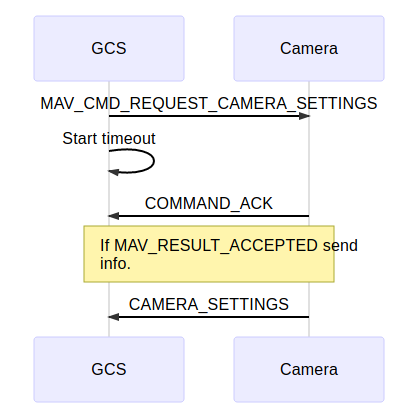
\includegraphics[scale=0.45]{img/camera_settings.png}
    \caption{Diagramme de demande de paramètres}
    \label{fig:CameraCmdsettings}
\end{figure}

Pour obtenir les paramètres de la caméra et savoir dans quel mode elle se trouve ( CAMERA\_MODE\_IMAGE ou CAMERA\_MODE\_VIDEO), le système maître doit envoyer la requête correspondante (MAC\_CMD\_REQUEST\_INFORMATION). La caméra transmet alors la structure suivante :

\begin{figure}[ht]
    \hspace{-2cm}
    {
        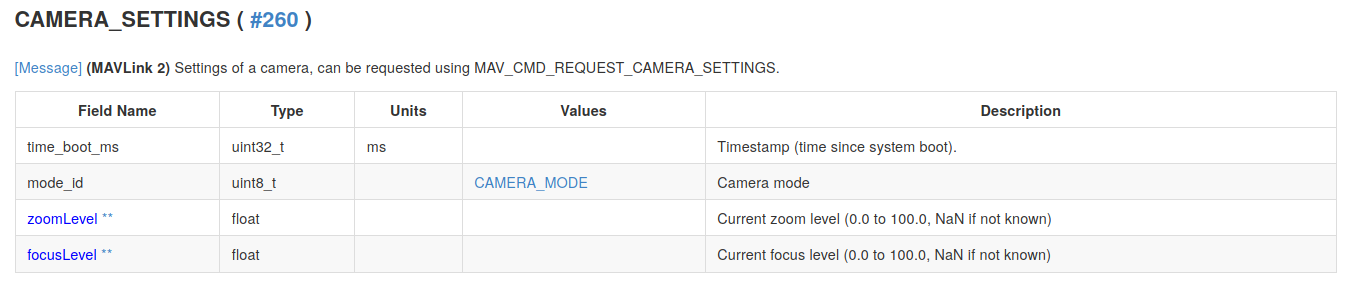
\includegraphics[scale=0.39]{img/settings_struct.png}
    }
    \caption{Champs des paramètres de la caméra}
    \label{fig:CameraCmdsetstruct}
\end{figure}
\newpage
\subsubsection{Set Camera Settings}
\begin{figure}[ht]
    \centering
    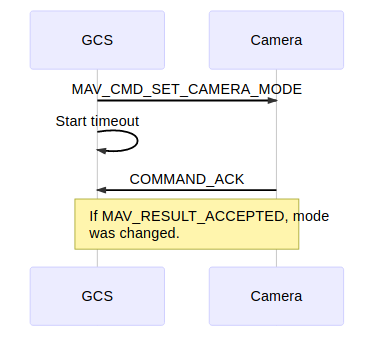
\includegraphics[scale=0.7]{img/camSetparams.png}
    \caption{Diagramme d'écriture du mode}
    \label{fig:CameraCmdsettings}
\end{figure}

Pour changer le mode d'une caméra( CAMERA\_MODE\_IMAGE ou CAMERA\_
MODE\_VIDEO), le focus et le zoom ,  la station de contrôle doit transmettre la commande suivante (MAC\_CMD\_SET\_CAMERA\_MODE). La caméra répond alors par un acquittement. 

\subsection{Camera Streaming}
La diffusion vidéo de la caméra peut être activée ou désactivée avec deux commandes MAVLINK.

\subsubsection{Camera Start Streaming}
MAV\_CMD\_VIDEO\_START\_STREAMING est la commande du protocole MAVLINK qui permet d'activer la caméra. Le flux de sortie vidéo ne passe pas par MAVLINK, il est géré indépendamment. 
Pour lancer un enregistrement vidéo, le dialogue suivant est établit : 
\begin{enumerate}
    \item La station de contrôle envoie MAV\_CMD\_VIDEO\_START\_STREAMING à la caméra. Cette commande contient en paramètre "StreamID". "StreamID" est un identifiant de streaming vidéos pouvant aller de 0 à n.
    \item La caméra répond à la commande par un acquittement qui peut contenir MAV\
    RESULT\_ACCEPTED ou MAV\_RESULT\_DENIED. 
\end{enumerate}
\subsubsection{Camera Stop Streaming}
MAV\_CMD\_VIDEO\_STOP\_STREAMING est la commande du protocole MAVLINK qui permet de stopper la diffusion vidéo.

Pour ce faire la commande MAV\_CMD\_VIDEO\_STOP\_STREAMING est transmise à la caméra et la diffusion vidéo est stoppée si l'acquittement émit par la caméra correspond à MAV\_RESULT\_ACCEPTED.